\documentclass[onecolumn, draftclsnofoot,10pt, compsoc]{IEEEtran}
\usepackage{graphicx}
\usepackage{url}
\usepackage{setspace}
\usepackage{listings}
\usepackage{xcolor}
\usepackage{caption}
\usepackage{subcaption}
\usepackage{float}

\usepackage{geometry}
\geometry{textheight=9.5in, textwidth=7in}

% Listings settings for swift taken from chriseidhof GitHub
\lstdefinelanguage{swift}
{
  morekeywords={
    func,if,then,else,for,in,while,do,switch,case,default,where,break,continue,fallthrough,return,
    typealias,struct,class,enum,protocol,var,func,let,get,set,willSet,didSet,inout,init,deinit,extension,
    subscript,prefix,operator,infix,postfix,precedence,associativity,left,right,none,convenience,dynamic,
    final,lazy,mutating,nonmutating,optional,override,required,static,unowned,safe,weak,internal,
    private,public,is,as,self,unsafe,dynamicType,true,false,nil,Type,Protocol,
  },
  morecomment=[l]{//}, % l is for line comment
  morecomment=[s]{/*}{*/}, % s is for start and end delimiter
  morestring=[b]" % defines that strings are enclosed in double quotes
}

\definecolor{keyword}{HTML}{BA2CA3}
\definecolor{string}{HTML}{D12F1B}
\definecolor{comment}{HTML}{008400}

\lstset{
  language=swift,
  basicstyle=\ttfamily,
  showstringspaces=false, % lets spaces in strings appear as real spaces
  columns=fixed,
  keepspaces=true,
  keywordstyle=\color{keyword},
  stringstyle=\color{string},
  commentstyle=\color{comment},
}

% 1. Fill in these details
\def \CapstoneTeamName{Manovacumeter Team}
\def \CapstoneTeamNumber{ 20}
\def \GroupMemberOne{Cade Raichart}
\def \GroupMemberTwo{Daniel Kato}
\def \GroupMemberThree{Nathan Shepherd}
\def \CapstoneProjectName{ISS Barometer App }
\def \CapstoneSponsorCompany{NASA}
\def \CapstoneSponsorPerson{Don Pettit}

% 2. Uncomment the appropriate line below so that the document type works
\def \DocType{Progress Report}

\newcommand{\NameSigPair}[1]{\par
\makebox[2.75in][r]{#1} \hfil 	\makebox[3.25in]{\makebox[2.25in]{\hrulefill} \hfill		\makebox[.75in]{\hrulefill}}
\par\vspace{-12pt} \textit{\tiny\noindent
\makebox[2.75in]{} \hfil		\makebox[3.25in]{\makebox[2.25in][r]{Signature} \hfill	\makebox[.75in][r]{Date}}}}
% 3. If the document is not to be signed, uncomment the RENEWcommand below
%\renewcommand{\NameSigPair}[1]{#1}

%%%%%%%%%%%%%%%%%%%%%%%%%%%%%%%%%%%%%%%
\begin{document}
\begin{titlepage}
    \pagenumbering{gobble}
    \begin{singlespace}
    	
\includegraphics[height=4cm]{coe_v_spot1}
        \hfill
        % 4. If you have a logo, use this includegraphics command to put it on the coversheet.
        %
\includegraphics[height=4cm]{NASA}
        \par\vspace{.2in}
        \centering
        \scshape{
            \huge CS Capstone \DocType \par
            {\large\today}\par
            \vspace{.5in}
            \textbf{\Huge\CapstoneProjectName}\par
            \vfill
            {\large Prepared for}\par
            \Huge \CapstoneSponsorCompany\par
            \vspace{5pt}
            {\Large\NameSigPair{\CapstoneSponsorPerson}\par}
            {\large Prepared by }\par
            Group\CapstoneTeamNumber\par
            % 5. comment out the line below this one if you do not wish to name your team
            %\CapstoneTeamName\par
            \vspace{5pt}
            {\Large
                \NameSigPair{\GroupMemberOne}\par
                \NameSigPair{\GroupMemberTwo}\par
                \NameSigPair{\GroupMemberThree}\par
            }
            \vspace{20pt}
        }
        \begin{abstract}
        % 6. Fill in your abstract
        The International Space Station, the conglomerate work of multiple national space associations, including NASA, requires precision devices to monitor the many aspects of space life.
        One very important aspect for the success of life in near vacuum is sustained air pressure inside the modules.
        This air pressure is monitored by mechanical barometers, called Manovacometers, which must be visually monitored, and are no longer available.
        The \CapstoneProjectName seeks to provide a suitable replacement for the current barometer device aboard the International Space Station.
        This document will update the reader on our progress, from the last Fall term Progress report.
        Each member has written their progress and plans, as well as a main refresher on our project as a whole.
        The member sections include Responsibilities, Current Status, Remaining Tasks, Problems Faced, and additional relevant or interesting details.
        This document should provide a clear picture of where the project stands, halfway through the Winter term, and halfway through the allotted year.
        \end{abstract}
    \end{singlespace}
\end{titlepage}
\newpage
\pagenumbering{arabic}
\tableofcontents
% 7. uncomment this (if applicable). Consider adding a page break.
%\listoffigures
%\listoftables
\clearpage

% 8. now you write!
\section{Project Purpose}
The ISS Barometer Application will be used on the ISS to measure and track air pressure.
The crew members aboard the ISS are currently reliant on mechanical barometers to take critical readings during leaks, or rapid depressurization events.
These leaks, caused by orbital debris, must be found and patched or the crew would need to evacuate.
Our application will improve on the mechanical barometers by providing clear and accurate pressure readings through the iPads on-board barometer sensor.
Readouts and measurements will be presented in a easy-to-read fashion that will allow users to quickly gauge the important details.
In further iterations, we plan to implement contextualized audio data readouts by using the t-Res document and a simple Swift api \cite{probStat}.

\section{Project Goals}
As mentioned above the application we are making will provide ISS crew members with an accurate and efficient pressure reading.
Our required features follow that purpose and are listed below:
\begin{itemize}
\item[V1:] Data Screen with initial pressure, current pressure, start/stop button, time stamp, pressure change (measured in sec / mmHg)
\item[V1:] Graph Screen with plot pressure as a function of time
\item[V1:] Additional settings menu that includes plot scale, scroll functionality, orientation, decimal point, as well as other other units of measure for pressure
\item[V1:] All items will be optimized for efficient reading and clear interface
\item[V2:] Graph will have pinch to zoom functionality, scaling options (to be set in settings)
\item[V2:] Graph will be able to be exported as a csv, excel readable file
\item[V2:] Graph can be compared to t-Res table, to measure time remaining
\item[V2:] Audio data readouts that will provide specific information at regular intervals
\end{itemize}

Along with these specific features, the application that we create must be efficient and clear, as decided by the users.
The application will be used in challenging situations and must be clear and easy to understand, so that the data can be conveyed quickly and without confusion.
From the listed project goals, we have sufficiently finished with V1, and have started implementing portions of V2, while trying to finalize our V1 progress.


% These sections can be used by whoever wrote them, I'm not sure who did which ones though

% \section{Project Problems}
% % Needs Rewritten
% We chose to use swift and Xcode because they allows for quick development and prototyping.
% This said we ran into many problems with that. For one Swift only works on Linux and MacOS.
% One of our group members did not have either at the time. They fixed this with installing a linux OS.
% Another problem was installing the swift libraries and connecting them with the Xcode application.
% Linux needed many packages to be downloaded for the library to work correctly, this took many hours of troubleshooting as it was not straightforward.
% Connecting swift to Xcode on the MacOS was another problem as well.
% Our last problem with swift and Xcode is we have no experience using either.
% We had and still have to continually work on improving our knowledge of these systems using online videos, guides and other resources.
%
% For the first time we all experienced what it was like working with someone who is in the workplace.
% We learned that our clients will not be getting back to us immediately and sometimes we have to wait for them reply.
% This means we have to work and finish our work and send it to him way earlier then we had planned originally.
% We also ran into the problems of finding the correct IEEE documentations.
% Sometimes we found the document quick and easy while other times it hours and many students combined to find them.


% We need to each write ~1000 words on our contributions
% Each of our sections could have interesting code, problems faced, issues managed
% I don't know really, but from the requirement this is the bulk of the writing

% Nathan- I've added sections for our bits. I think we can fill in Responsibilities with just the
%           issues we've taken for gitHub, I just copy and pasted them in including ones that I had a part in.
%
\section{Specific Contributions: Daniel Kato}
    \subsection{Responsibilities}
    I started the development process by creating a base project with the Charts API installed, and creating a main view and settings view in the storyboard.

        For the chart I got a blank chart up and running on the display.
        This involved binding the Charts API's \texttt{LineChartView} class to a subview on the Main UI.
        I also created a view controller for that view called \texttt{ChartViewController} to control what is drawn in the \texttt{LineChartView}.
        I configured the chart to display according to Nathan's color palette and made some small changes to the way the chart was drawn.
        In order for the chart to access the barometer data, I created a function in the \texttt{ChartViewController} called \texttt{updateChart} to be called every time a reading is taken with the pressure and time of the reading.
        This allowed me to move on and implement the live updating functionality of the chart.

        For the main UI, I added all of the readings, timestamps, labels, and buttons to the UI as well as implemented the logic that supplied the values to each.
        In the middle of connecting all of the moving parts, I decided to abstract the barometer functionality into its own class so the the code could be more readable.
        I also configured the UI to use a Navigation Controller to manage switching to the settings view.

        For the settings UI, I added the table view holding all of the settings interfaces as well as the units, significant digits and orientation rows.
        I also implemented the functionality for changing the units that are displayed on the readings and the chart by creating a settings class which is instantiated once and referenced by each view.
        This allows the selected unit can be saved as a string in the settings object, and when switching back to the main view, the unit string is read from the object.
        The converting of chart points is done in a handler function that responds to a button tab being pressed.
        I also implemented the significant digits and orientation logic in a similar way to the units.

        All of my code contributions have been kept track of by github issues, which are detailed below.

        \begin{itemize}
        \item Add button to record average dP/dt and dt/dP since last press or start of data
        \item Add 3rd column with avg dP/dt and avg dt/dP
        \item Adjust Delta with conversion bug fix
        \item Convert past data points when a unit is picked
        \item Save settings to coreData when app is terminated
        \item Add Reset Delta Button
        \item Adjust Axes on Chart
        \item Change Delta Pressure functionality
        \item Add delta time to Main UI
        \item Add current time to Main UI
        \item Make x-axis of chart display the time of the reading
        \item Abstract barometer functionality into its own class
        \item Test Pressure Display
        \item Remove labels from bottom of chart
        \item Chart updates, but data is not shown
        \item Construct Chart
        \item App Icon
        \item Linked Barometer Data to Chart
        \item Unit Picker Button
        \item Orientation Setting Button
        \item Figure out how to add barometer data to graph
        \item Significant Digits Button
        \end{itemize}

    \subsection{Current Status}
        We are currently updating the UI and adding a few features that Don requested in response to seeing our alpha version of the app.
        This alpha version includes a main UI with readings of current pressure and time, change in pressure since button press and time of press, average $\frac{\Delta p}{\Delta t}$ and $\frac{\Delta t}{\Delta p}$ since button press and time of press, and a chart of pressure over time.
        The delta reading has a corresponding button that when pressed updates the display with the change in pressure since the last time the button was pressed.
        Similarly, the average $\frac{\Delta p}{\Delta t}$ and $\frac{\Delta t}{\Delta p}$ readings have a corresponding buttons that when pressed updates the display with the average $\frac{\Delta p}{\Delta t}$ and $\frac{\Delta t}{\Delta p}$ since the last button press.

        The chart is currently displays the current pressure as a function of time with the ability to pinch to zoom.
        The x-axis displays the time of the reading in the format determined for the system in the system settings app.
        Whenever the units for the graph are changed, the y-axis points are converted to reflect the new unit of measurement while maintaining the shape of the graph.

        The settings page currently allows for the configuration of units, significant digits, orientation, and graph style.
        The available units are mmHg, psi, kPa, and atm.
        The significant digit allow for between 0 and 10 significant digits.
        The orientation allows for the orientation to be up, down, left, or right compared to the default orientation (camera above display and home button below).

    \subsection{Remaining Tasks}
        The application still needs to include axis labels, and have the UI updated, before having a complete alpha version.
        Once the alpha has been accepted, we will incorporate the existing T-res chart into our application as well as a reading that displays the amount of time before an evacuation is necessary.
        We will also incorporate a vocal readout of the amount of time left, and the ability to lock the screen from touch input unless a lock icon is pressed again.
        We also need to redesign the app icon to depict the ISS with a hole in it with air escaping.

    \subsection{Problems Faced}
        One of the problems I ran into was getting the orientation to lock.
        There was not much information on the web about programmatically locking the orientation in Swift 4.
        I eventually found out that you can set the orientation with a call to \texttt{UIDevice.current.setValue(<orientationInt>, forKey: "orientation")}.
        Also, we switched from placing UI elements by dragging and dropping them in the appropriate location, to using Stacks to stack items so they can be automatically adjusted to fit the orientation/device.
        In the transition to stacks, we ran into issues with centering certain elements.

    \subsection{Relevant and Interesting Details}
        After completing the settings UI, we needed the settings to persist from use to use.
        To solution to this problem was UserDefaults which allows you to store serialized objects and retrieve them by an ID later is the class conforms to the \texttt{Codable} class.
        The code to implement this was very easy to read and implement and is as follows:

\begin{lstlisting}
// Settings Object
class Settings: Codable {
    var units = "mmHg"
    var sigFigs = 4
    var orientation = "Right"
    var slidingScale = false
    var slidingScaleThreshold = 20
    var windowSize = 50
}

// Store Settings Object
UserDefaults.standard.set(try? PropertyListEncoder().encode(settings), forKey: "Settings")

// Retrieve Settings Object
func application(_ application: UIApplication, didFinishLaunchingWithOptions launchOptions: [UIApplicationLaunchOptionsKey: Any]?) -> Bool {
    if let data = UserDefaults.standard.value(forKey: "Settings") as? Data {
        settings = try? PropertyListDecoder().decode(Settings.self, from: data)
    }
    if settings == nil {
        settings = Settings()
    }
    return true
}

\end{lstlisting}


\section{Specific Contributions: Cade Raichart}
\subsection{Responsibilities}
My first task for the project was to create the settings page using Daniels \texttt{viewController} that he prepared in advance.
I created  a unit picker, which was a pull down menu that allowed the user to choose between mmHg, atm, kPa and PSI.
Then I created a significant digit picker that lets the user pick up to ten significant digits, using a scroll bar.
Next I worked on orientation.
I attempted to format the screen so that it would lock and then rotate in a chosen direction.
I was  unsuccessful so I collaborated with Daniel, who ended up finding the solution.
We decided to remove my unit picker and significant units, and instead agreed on a simpler design.
After we showed our alpha version to our client, he asked us to make some changes.
I removed the labels that said “timestamp” leaving only the clock.
I also increased the font so that those who are visually impaired could clearly read it.
Finally, I  formatted the rest of the labels and digits, so that they were all aligned, making them more neat and organized.

My contributions:
\begin{itemize}
\item Unit Picker
\item Significant Units
\item Orientation
\item Take away Timestamp
\item Make all numbers and labels bigger
\item Make all Labels fit on page with equal spacing
\item Make all Labels look pleasing to the eye
\end{itemize}

\subsection{Current Status}
We are finishing up the newest requests that our client has requested after seeing our latest alpha.
These additions are making the display page more readable and organized, including labels on the graph and bigger digits for reading.

The alpha version included a display page and a settings page.
The display page included a current pressure, change in pressure(Delta), average change in pressure over time, average change in time over change in pressure, and lastly a running graph.

The change in pressure display has a button that starts displaying the Delta, which represents the change in pressure from the last time it was pressed to the current time.
This also leaves a timestamp.
Both $\frac{\Delta p}{\Delta t}$ and $\frac{\Delta t}{\Delta p}$ have a button that starts recording the values and also leaves a timestamp.

The running graph displays pressure vs time.
Pressure is represented on the y-axis while time is represented by the x-axis.
This graph allows the user to zoom in by pinching the screen.
The x-axis will change its format of display when the internal ipad settings are changed, while the y-axis will changes its units when the units are changed in the settings page.

The settings page includes a units picker, significant digits slider, an orientation picker, and a graph style.
The unit picker allows the user to pick between atm, mmHg, PSI and kPa.
Our slider allows up to ten significant digits.
Our screen orientation is locked by default but allows users to reorient the screen however they choose.
Last, the graph style allows the user to choose the sliding scale and the window size.

\subsection{Remaining Tasks}
The next step of our project is to begin work on version two.
Our client has asked us to add dictation as well as T-Res tables.
T-Res is tables of data points that tell us the amount of pressure that would cause the crew to need to leave the ship vs how fast the pressure is dropping.
The faster the pressure is dropping the earlier the crew needs to evacuate the space station.
These tables will be implemented into our program so that we can dictate a countdown for evacuation.
Lastly our client has asked us to add the option to lock the screen to touch.

Version two features:
\begin{itemize}
\item Dictation
\item T-RES tables
\item Lock screen
\end{itemize}

We will use T-Res tables provided by our client and our app will dictate these numbers.
It will also be able to dictate the display numbers, such as current pressure, in the event that the crew members cannot read the display.
I have already started testing on how we can use the library AVFoundation to easily add dictation to our app.
Finally, we will have our client view our product again and decide if more features should be added, or if changes need to be made to the display.

\subsection{Problems Faced}
The biggest problem I faced was locking the orientation and then being able to reorient the display to the users’ preferences.
I spent hours searching the web for help and mostly came up with ideas that just didn't work such as:

\begin{lstlisting}
static func lockOrientation(_ orientation: UIInterfaceOrientationMask, andRotateTo rotateOrientation:UIInterfaceOrientation) {self.lockOrientation(orientation)}
\end{lstlisting}

    I found a lot of code like this one that potentially could have worked, but when implemented didn't lock the screen or allow you to switch your orientation.
    In fact, most research told me i could use the code “ self.lockOrientation(left)” to lock the screen but i was unsuccessful.
    Daniel and Nathan ended up helping me with this problem and found {UIDevice.current.setValue(<orientationInt>, forKey: "orientation")} to fix the orientation, so that the user could orient the screen however they wanted.

    Another problem I faced was orienting the stacks so that they were all aligned.
    There were no instructions on how to use the \texttt{viewController} stacks online, so I had to manually adjust the stacks until I found a solution.
    This solution was using more stacks within each other and making sure every single stack was correctly aligned with the previous one.

\subsection{Relevant and Interesting Details}

The most interesting thing i have found is how viewcontrollers are easy to use for simple programs because swift and Xcode have made it easy to drag and drop items.
However, viewcontrollers create an organization problem for more in depth programs, because these items easily overlap making them hard to move.
We started to use stacks that allowed us to make it easier to group items together and make them less cluttered.
Although the \texttt{viewController} is useful for small apps, if this app were more extensive I would try to avoid the use of the \texttt{viewController} and remove it from the program.


\section{Specific Contributions: Nathan Shepherd}

\subsection{Responsibilities}

From the technology document, I was tasked with the general projects of language choice, data storage, and color palette.
In those sections, I chose Swift, NSUserDefaults, and a self-defined blue theme.
Although these choices made significant impact on our design process, they didn't provide many facets of work.
The language choice affected all teammates, and was in fact already chosen at the start of the project.
The data storage is more complicated, and does have work involved with it; but that work was done by another teammate, as it aligned better with their past contributions.
The color palette turned out to be more restrained than expected, as the users have strict needs for readability and clarity.
This meant that our lettering and icons were required to be black on white background, for visibility, and only our banners and the application icons were altered.
Due to the technologies being vague and rather non-actionable, the team stuck to GitHub issues as our means of delegation.
As follows, these are the issues I took both full and partial responsibility for:

\begin{itemize}
  \item Adjust Y-Axis Default Zoom
  \item Random Debug Data
  \item Unit Picker Setting
  \item Rolling graph Setting
  \item Adding X-axis and Y-axis titles
\end{itemize}

\subsection{Current Status}

Currently our application is a fully functional prototype with near full coverage of our version one goals.
It properly records air pressure, and displays a graph, along with the requested current pressure, $\frac{\Delta p}{\Delta t}$, and $\frac{\Delta t}{\Delta p}$.
In addition we have implemented the following settings, and initialized them with assumed defaults:

\begin{lstlisting}
class Settings: Codable {
    var units = "mmHg"
    var sigFigs = 4
    var orientation = "Right"
    var slidingScale = false
    var windowSize = 50
}
\end{lstlisting}

These settings allow the user to change and save their preferences, making the application more interactive.
The units that can be chosen are mmHg, psi, kPa, and atm.
The changes then propagate to both the data view and the plot, making both scale appropriately.
The significant figure setting can be incremented anywhere between 0 and 10.
The orientation is a user setting because, as described in our requirements document, the iPad accelerometer doesn't work very well in the microgravity of the ISS.
To solve this the orientation is fixed, and can be changed by the user manually.
The sliding scale is a switch that will allow the user to choose between two graph functions: The first and default, is a scaling graph, that shrinks with more data; the second is a graph with a set window size, and will follow new data as it's returned.
The set window size option, if selected, will reveal a window size slider that allow the user to choose the size of the rolling window.
In addition to specific user settings, I have implemented a stream of debug data, when an on board barometer isn't available.
This will be removed before our final release, but it allows us to test the application just by running it on the Xcode emulator.

\subsection{Remaining Tasks}
The majority of remaining issues that we have to face are either UI adjustments, or version two features.
The UI adjustments include making the labels both larger and more readable, and adjusting the axis labels further (more info in the next section).
The client has also added some functionality to the version two release which include the following:

\begin{itemize}
  \item Dictation
  \item Screen lock
  \item T-Res Alarm
\end{itemize}

These issues will not be out of scope, and shouldn't be difficult to implement.
The dictation will include regular audio readouts of the pressure and pressure rates.
The interval and detail of these readouts have yet to be determined, but by implementing an internal text-to-speech Swift interface, the dictation should be quick to introduce and provide a hands free solution in the case of an emergency.

\subsection{Problems Faced}

The problems faced involved my efforts on rolling screen functionality and axis titles.
The rolling screen functionality was the setting that allowed users to select the charts display mode.
To implement rolling screen I had to set the minimum and maximum x axis for each data point added.
It was simple enough to write this functionality but to make it call at regular intervals proved trickier.
The solution I implemented was a timer object, that would activate each second, similar to the barometer polling.
This allowed for the settings that affected the barometer, such as the units, to also change the debug data.
The issue caused by the axis titles is still causing trouble.
It comes from the fact that as a team, we want to have axis aligned titles, with the y-axis title being vertically orientated.
It is only a single command that rotates the label, and is not really a challenge, but once rotated, Xcode's auto-formatting no longer applies.
This means that size constraints that are applied before the rotation of the label are, for the most part, disregarded, as shown in the images below in fig \ref{fig:comparison}.

\begin{figure}[H]
\centering
\begin{subfigure}{.5\textwidth}
  \centering
  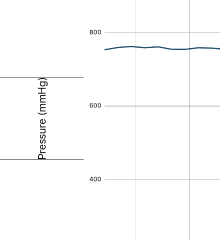
\includegraphics[width=.4\linewidth]{widthAxis}
  \caption{Label with width constraints}
  \label{fig:width}
\end{subfigure}%
\begin{subfigure}{.5\textwidth}
  \centering
  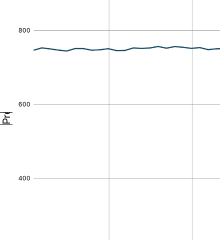
\includegraphics[width=.4\linewidth]{heightAxis}
  \caption{Label with height constraints}
  \label{fig:height}
\end{subfigure}
\caption{A comparison of constraints on y axis label.}
\label{fig:comparison}
\end{figure}

By fixing the width, the location of the label is affected, making the margin a ridiculous waste of space.
When I try to fix this issue by also fixing the height of the label, the result is a truncated label.
The solution that I was able to arrive at involved changing the implemented workspace technique, of using \texttt{Stacks}, to now using \texttt{Views}.
This allows for more detailed adjustments, making it possible to constrain labels with position, and not just size.
The result, shown in fig \ref{fig:comparison}, is the current solution.
By using the following code, I am able to adjust the size of the label, after it is rotated.

\begin{lstlisting}
func adjustAxisLabels() {
    yAxisLabel.transform = CGAffineTransform(rotationAngle: -CGFloat.pi/2)
    yAxisLabel.text = "Pressure (\(settings.units))"
    yAxisLabel.sizeToFit()
}
\end{lstlisting}

\begin{figure}[H]
  \centering
  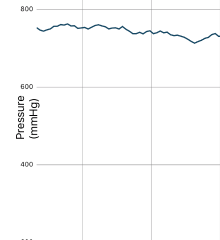
\includegraphics[width=.3\linewidth]{solution}
  \caption{The current solution of the label issue.}
  \label{fig:solution}
\end{figure}

\subsection{Relevant and Interesting Details}

The main interesting detail that I've noticed in my parts of the project is the difficulty of rotated titles.
I'm sure that it has been established, but the complications that I have encountered in dealing with the labels has surprised me.
Another thing that interested me was the adaptions requested for use aboard the ISS.
I think that the applications use in microgravity and emergency situations is the most interesting detail of this project.
The adaptions include things like the locked orientation and audio readout, as well as large font and clear typeface choices.
It will be particularly interesting to deploy our application and hear feedback from real users.

\section{Conclusion}

We are currently waiting on feedback from our users, the astronauts, but from where we stand now the conclusions are as follows.
Our application quickly and accurately displays the reading and analysis of pressure data, as requested.
By using the application, the astronauts will be able to find and repair leaks with added safety, reliability, and speed.
With the potential to continue improving, this application may very well serve NASA far into the future.
Taking into account our progress so far, it seems reasonable to assume that our project will succeed and fill the requirements that were set out.
​

\newpage
\bibliographystyle{IEEEtran}
\bibliography{bibliography}
\end{document}
